\section{Tagging algorithms and Operating Points}
\label{sec:taggingalgos}
Several algorithms to identify jets originating from 
the decay of a $b$ quark are available in CMSSW. The ones considered in this 
analysis rely on the extended lifetime of B hadrons. In particular, the 
TrackCounting and the JetProbability taggers rely on tracks with large impact 
parameters with respect to the interaction point. 

The TrackCounting tagger (TC) computes the impact parameter significance 
$IP/\sigma_{IP}$ for each selected track in a jet. The jet is tagged as a 
$b$ jet if the number of tracks with an $IP/\sigma_{IP}$ exceeding a given 
cut is greater than a value which can be optimized for high efficiency or
high purity in the resulting sample. Tracks are ordered in decreasing 
impact parameter significance $IP/\sigma_{IP}$. The significance of the track
impact parameter of the $N^{th} $ track serves as the discriminator for this 
algorithm.
In this note, two discriminants were chosen for the TrackCounting tagger by 
requiring second ($TCHE$) or third ($TCHP$) track with a 3D $IP/\sigma_{IP}$ 
larger than a given cut.

The JetProbability tagger (JP) is also based on track impact parameter:
it computes how likely it is for a set of tracks to have originated from the 
primary vertex, based on the $IP/\sigma_{IP}$ of each track in a jet. 

Figure ~\ref{fig:Performance_plots} shows the tagging efficiencies for $c$ and 
light jets as a funcion of the efficiency to tag a $b$ jet, as measured  
using the Monte Carlo truth information to identify the flavour of a 
particular jet in the QCD $80<\hat{p_T}<120\;{\rm GeV}/c$ sample. 

Based on this study, three operating points are defined that select 
an average fraction of approximately 10\%, 1\% or 0.1\%, 
respectively, of $udsg$ jets in the QCD 80-120 sample.
Table~\ref{tab:OperatingPoints} summarizes 
the definition of the operating points.

\begin{figure}[htbp]
  \begin{center}
    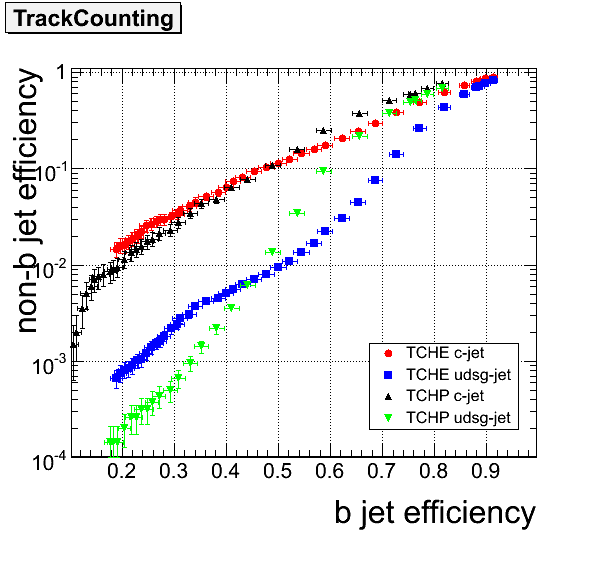
\includegraphics[width=60mm]{Figures/Performance_plot_TC.png}
    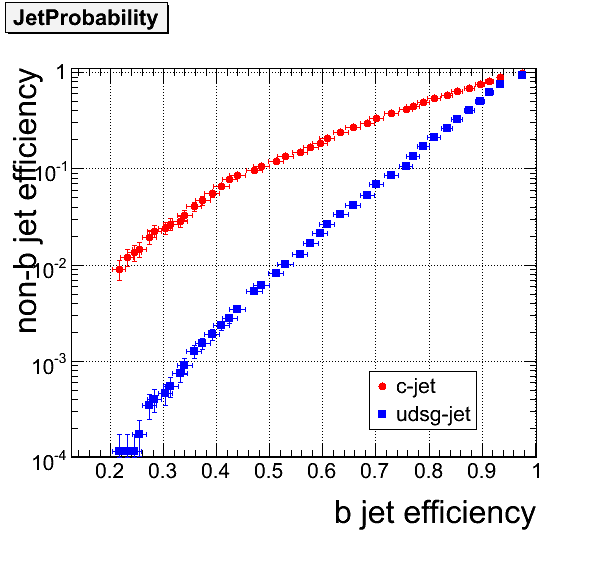
\includegraphics[width=60mm]{Figures/Performance_plot_TP.png}
  \end{center}
  \caption{b-tagging performance measured using the MC truth information 
on the QCD sample with $80<\hat{p_T}<120\;{\rm GeV}/c$ for the TrackCounting 
(left) and the JetProbability tagger(right).}
  \label{fig:Performance_plots}
\end{figure}

\begin{table} [th]
\begin{center}
\begin{tabular}{|l|c|l|c|} 
\hline
Algorithm         & Discriminator & Algorithm      & Discriminator\\ \hline
Track Counting    &               & JetProbability &              \\
Loose  (TCL)      &  $TCHE>2.0$   & Loose  (JPL)   &  $>0.26$\\ 
Medium (TCM)      &  $TCHE>4.6$   & Medium (JPM)   &  $>0.50$\\ 
Tight  (TCT)      &  $TCHP>4.7$   & Tight  (JPT)   &  $>0.76$\\ 
\hline
\end{tabular}
\caption{\label{tab:OperatingPoints} 
 Operating points for the TrackCounting and the JetProbability algorithms,
 determined  from MC truth, for jets with $p_T>20$~\gevc and $|\eta|<2.5$.}
 \end{center}
\end{table}
